\chapter{The \locate* step}
\label{chap:locate}

\newcommand{\locateimgsize}{0.9\textwidth}

The task of the \locate* step consists in extracting the positions of the bubbles in pixel coordinates, independently for each frame of each camera.

\section{Requirements}

\subsection{Input}
The \locate* step receives as input the videos captured by the cameras, frame by frame.
The images are pre-processed by an FPGA included in the cameras: the background is removed, and the resulting image is binarized with a threshold, to have distinct white bubbles over a black background.
Figure~\ref{fig:locate:original} depicts an example input frame.

\begin{figure}
	\centerline{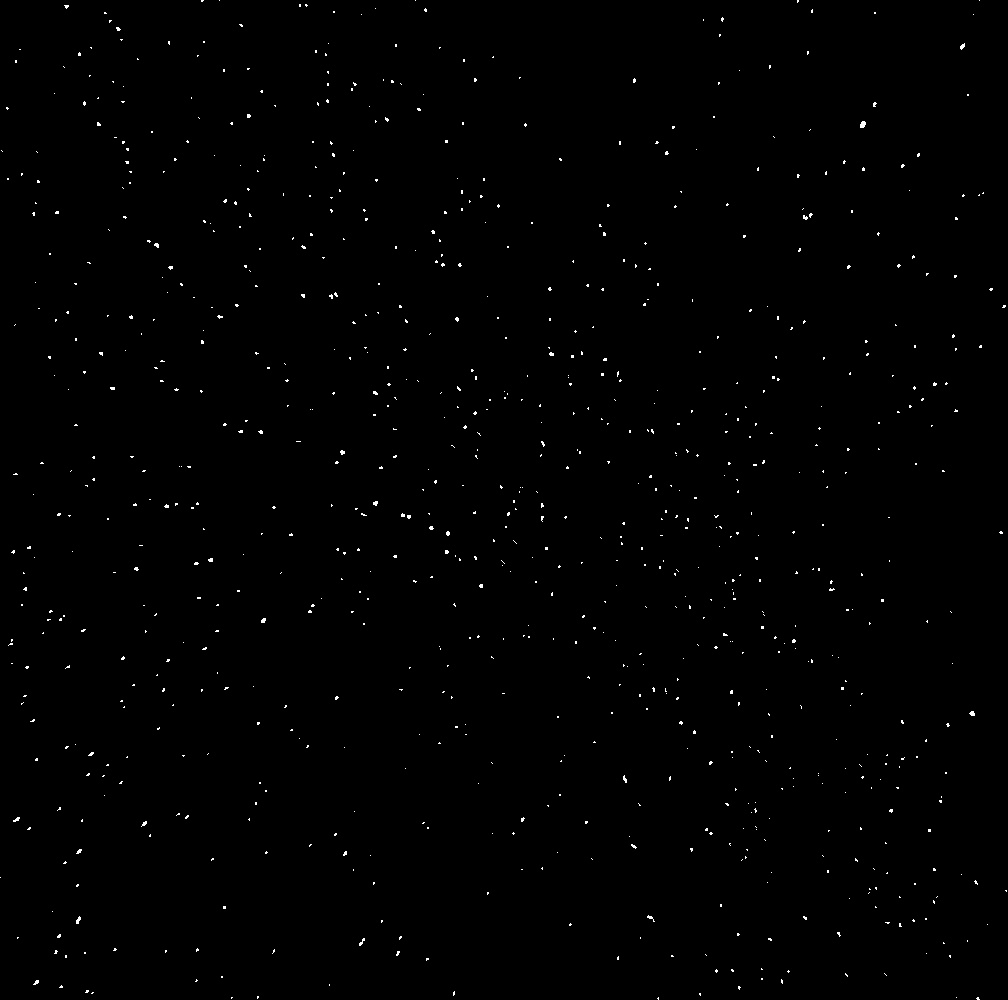
\includegraphics[width=\locateimgsize]{images/locate/_original-frame-full.png}}
	\caption{\centering An example of frame returned by the cameras}
	\label{fig:locate:original}
\end{figure}

\subsection{Output}
\label{sec:locate:output}

The output of the \locate* step is a couple of \texttt{numpy} arrays.
An array called \texttt{positions} describes the coordinates of each bubble present in a frame.
It is a four-dimensional, floating-point array, where \texttt{positions[C][F][B]} describes the $B$-th bubble of the $F$-th frame of camera $C$, in the form of an \texttt{(x, y[, area])} tuple.
Bubbles are ordered in a random, arbitrary way for each frame: there is no correlation between two bubbles with the same $B$ but different $C$ and/or $F$.

Due to \texttt{numpy} limitations, the array is pre-allocated of a fixed size: while the number of cameras is fixed, an upper limit on the number of frames and bubbles must be decided before execution.
Knowing which frames contain meaningful data is trivial, while it is not for the number of bubbles, that can change between frame and frame.
For this reason, a second array was introduced: \texttt{numTracers} is a two-dimensional, integer array.
\texttt{numTracers[C][F]} carries the information of how many tracers are valid inside the $F$-th frame of camera $C$.
The coordinates of the valid tracers will therefore be \texttt{positions[C][F][numTracers[C][F]]}.

\subsection{Speed}

When used on a setup of $N$ cameras with frame rate $f$ each, the \locate* step would receive $N{\cdot}f$ independent frames each second.
To respect the real-time constraint, the \locate* step would therefore need to operate at a minimum of $N{\cdot}f$ FPS.

When I did the analysis on the \locate* step, the plan was to have 3 cameras working at 30 FPS, requiring a 90 FPS \locate* step.
Later, the cameras turned out to be slower, at 24 FPS, but there were 4: the final \locate* implementation was able to manage also these 96 FPS.

\subsection{Quality}

Ideally, all tracers should be detected, since errors in the locating process would propagate to future steps:
\begin{itemize}
	\itemsep 0em
	\item \textbf{False positives}: the \match* phase will have more candidates, leading to \textit{possible} wrong reconstructions: the \match* can both choose the correct bubble, or the one added by the error (or another real one);
	\item \textbf{False negatives:} the same bubble in another frame will not have the correct match, leading to \textit{certain} wrong reconstructions.
\end{itemize}
As such, it is better to overpredict (false positives) than to miss bubbles.

It is however to be noted that the most important requirement is the speed: a worse implementation which is speedwise above target should be preferred to a better implementation that does not meet speed requirements.

\section{State of the art}

When searching on the Internet some existing solutions to perform the \locate* task, the following approaches were found:
\begin{itemize}
	\itemsep 0em
	\item The Trackpy~\cite{trackpy} Python library (evaluated in section~\ref{sec:locate:trackpy});
	\item The MyPTV~\cite{myptv} Python library (evaluated in section~\ref{sec:locate:myptv});
	\item The TracTrac~\cite{tractrac} Python program (evaluated in section~\ref{sec:locate:tractrac});
	\item The 4d-ptv~\cite{fourdptv} Matlab script (evaluated in section~\ref{sec:locate:fourdptv}).
\end{itemize}
In the aim of finding the best approach, the listed algorithms were evaluated in the same way as novel algorithmic ideas.
In some cases, potential weaknesses in the algorithm were found: some of the new approaches developed within this thesis are therefore evolutions of these algorithms.
For this reason, their description and evaluation is in the following chapters.

\section{Approaches}
\label{sec:locate:approaches}

The following sections describe the many different approaches evaluated for the \locate* step.
Their speed and quality is compared on a common 1-camera, 100-frame sequence.
Each approach reports an example frame: it is the result of performing the \locate* on figure~\ref{fig:locate:original-crop}, which itself is a portion of the frame in figure~\ref{fig:locate:original}.

\begin{figure}[H]
	\centerline{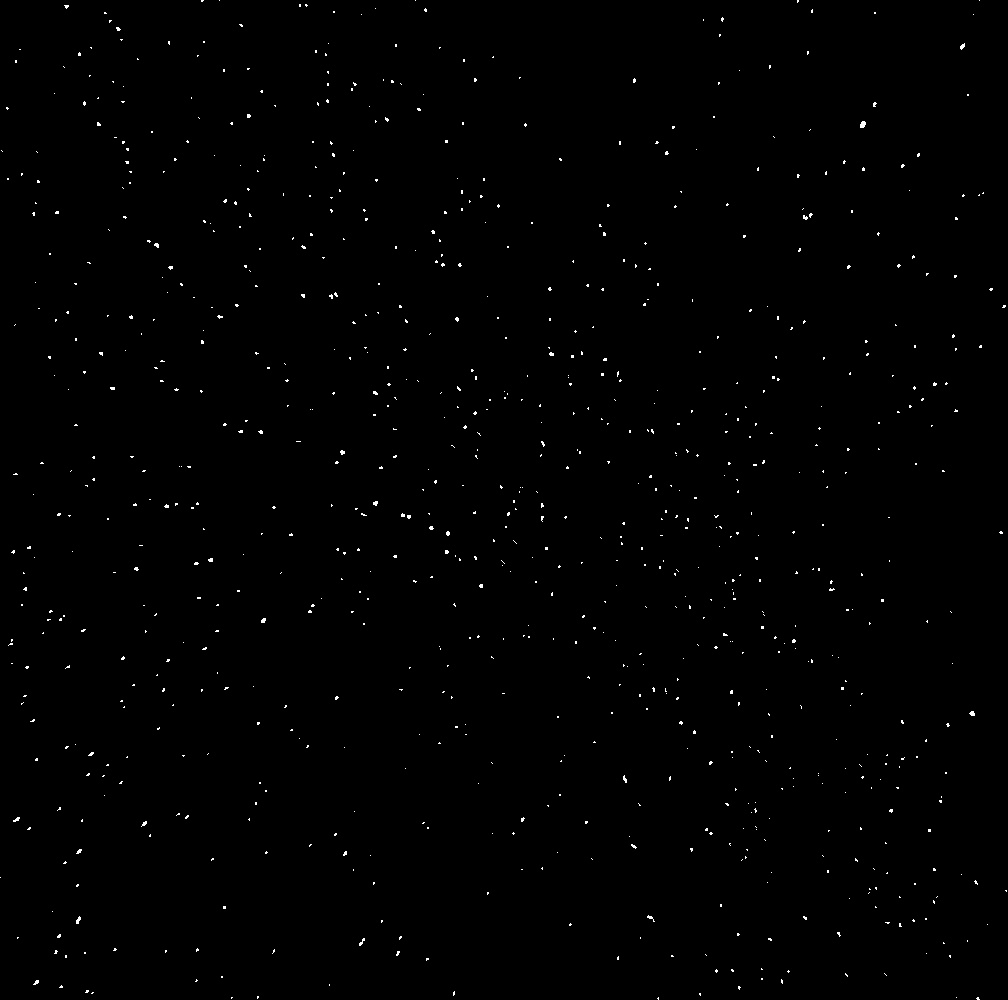
\includegraphics[width=\locateimgsize]{images/locate/_original-frame.png}}
	\caption{\centering The portion of figure~\ref{fig:locate:original} used to display the locate result}
	\label{fig:locate:original-crop}
\end{figure}


\newpage
\subsection{Trackpy}
\label{sec:locate:trackpy}

Trackpy~\cite{trackpy} is a particle tracking library developed by Soft Matter.
Its \texttt{Locate} function performs the task required, if an extra output format transformation step is applied.

\subsubsection{Algorithm}

As described in the documentation, the \texttt{Locate} function implements the following algorithm:
\begin{enumerate}
	\itemsep 0em
	\item Pre-process the image by performing a band pass and a threshold.
	\item Locate all peaks of brightness, characterize the neighborhoods of the peaks and take only those with given total brightness (``mass'').
	\item Refine the positions of each peak.
\end{enumerate}

\subsubsection{Evaluation}

As displayed in figure~\ref{fig:locate:trackpy}, the algorithm performed well on quality, finding about 85\% of the tracers.
The speed was however extremely low, at just 3 FPS.

\begin{figure}
	\centerline{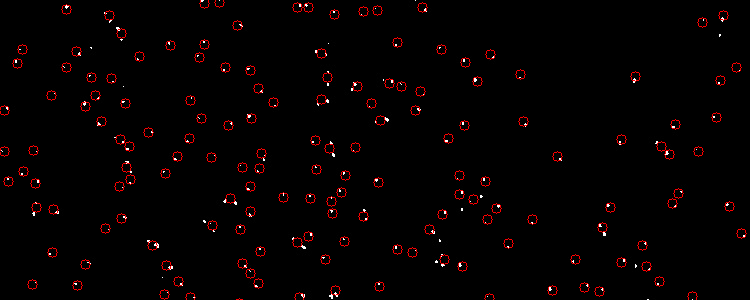
\includegraphics[width=\locateimgsize]{images/locate/trackpy.png}}
	\caption{\centering Trackpy's result}
	\label{fig:locate:trackpy}
\end{figure}
 \newpage
\subsection{Trackpy (CuPy)}

When profiling the Trackpy code, the functions \texttt{fourier\_gaussian}, \texttt{uniform\_filter1d} and \texttt{correlate1d} from \texttt{SciPy} took a considerable amount of time.
For this reason, Trackpy's code was altered to use the \texttt{CuPy} library instead of \texttt{SciPy} for these operations.
This aimed to exploit the GPU for faster computation.

\subsubsection{Algorithm}

The algorithm is the same as Trackpy's, with some extra steps required to transfer the various arrays to/from GPU memory.
These transfers were reduced to the minimum, to reduce the overhead as much as possible.

\subsubsection{Evaluation}

Figure~\ref{fig:locate:trackpy-cupy} shows the result, which for unknown reasons is different than Trackpy's: it lost the offset problem, but the percentage of identified bubbles reduced to 79\%.
Speedwise, the algorithm is slightly faster, running at 7 FPS: still extremely far from the target.

\begin{figure}
	\centerline{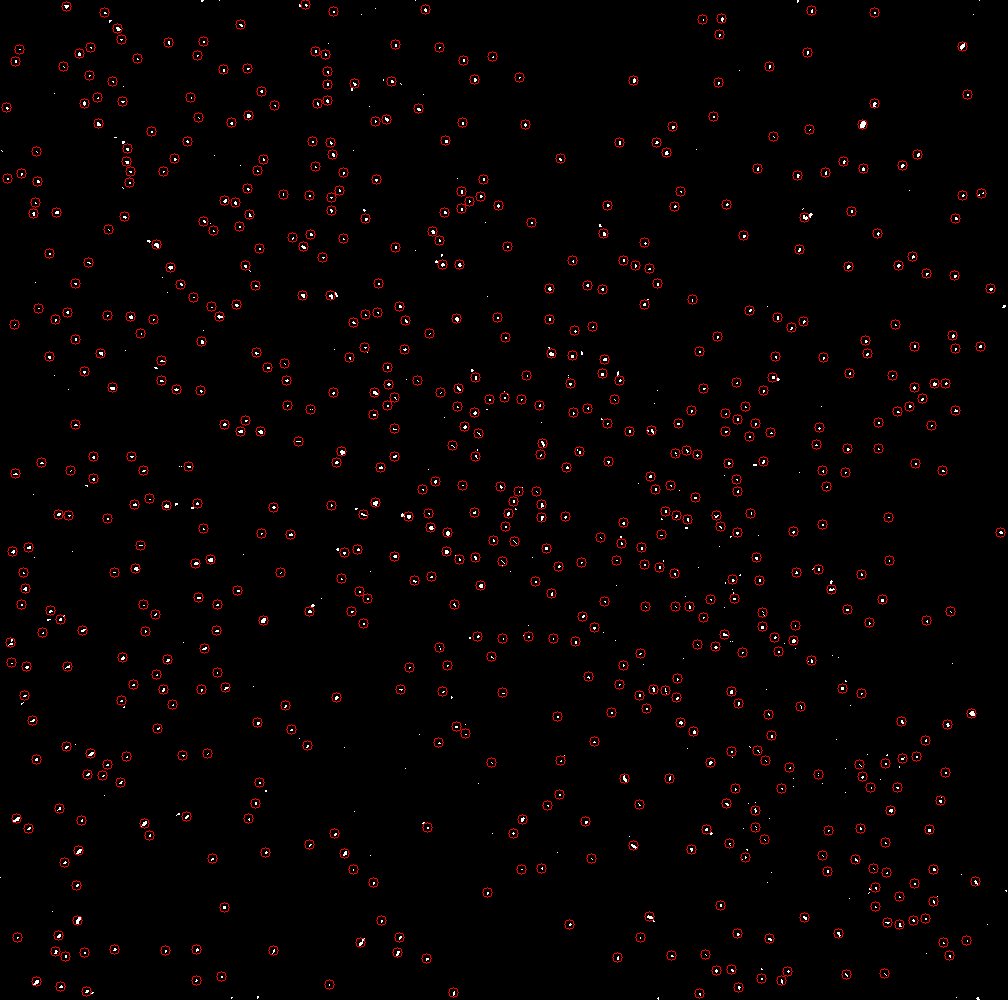
\includegraphics[width=\locateimgsize]{images/locate/cuda-trackpy.png}}
	\caption{\centering Trackpy with CuPy's result}
	\label{fig:locate:trackpy-cupy}
\end{figure}
 \newpage
\subsection{CNN}

The task of \textit{finding the coordinates of the bubbles} can be seen as \textit{for each pixel, check if it is the center of a bubble}.
The task of looking for the same thing across all pixels of an image is the foundation of image convolution and convolutional layers in neural network.
As such, a SAME CONV neural layer was proposed, with a kernel size big enough for containing a full bubble.
The CNN would transform the input image into a binary image, where ``on'' pixels would represent bubble centers.

\subsubsection{Algorithm}

\begin{itemize}
	\itemsep 0em
	\item Initially, the single-layer CNN evaluates the image, to find centroids of the bubbles;
	\item At a second stage, a loop would collect all the ``on'' pixels of the image into a list of coordinates.
\end{itemize}

\subsubsection{Evaluation}

Initially, only a feasibility study was performed: the CNN was trained with just a single epoch of 8 images, to evaluate if the inference speed was good enough to justify a longer training.
The result shown in figure~\ref{fig:locate:cnn} is promising for the little training performed, but it clearly needs more refinement.

Most importantly, the speed was much greater than the previous ones, at 55 FPS, but still far from the target.
As such, further approaches would be evaluated before performing a deeper training, to investigate if a greater speed was achievable.

\begin{figure}
	\centerline{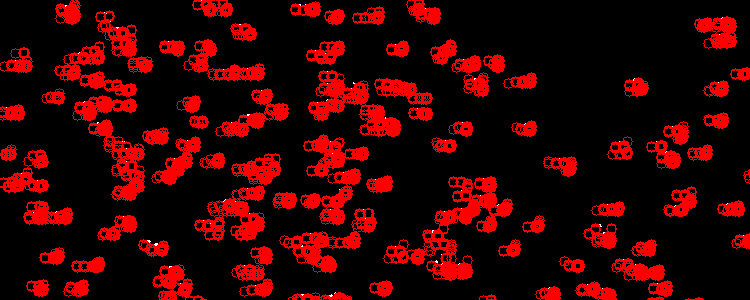
\includegraphics[width=\locateimgsize]{images/locate/cnn.png}}
	\caption{\centering The CNN's result}
	\label{fig:locate:cnn}
\end{figure}
 \newpage
\subsection{Torch.unfold concept}
\label{sec:locate:torchunfold}

The \texttt{unfold} function from \texttt{PyTorch} takes an image, and breaks it into either disjoint or partially overlapping tiles.
The idea is to use a divide and conquer approach, where the full image is split into smaller images, hopefully making it faster.


\subsubsection{Algorithm}

The overall algorithm divides the image into patches, to then process each one separately.
Different tile sizes were compared, to find the best, if any.

\subsubsection{Evaluation}

As visible in table~\ref{tab:torch.unfold}, having smaller patches increases the time required to perform the overall \locate*.
This is likely due to the overlap between patches.
The overlap is however necessary, to avoid bubbles split across patches to be considered as separate.

\begin{table}[ht]
	\centering
	\def\arraystretch{2}
	\begin{tabularx}{\linewidth}{
		|>{\arraybackslash}p{.2\linewidth}
		|>{\centering\arraybackslash}X
		|>{\centering\arraybackslash}X
		|>{\centering\arraybackslash}X
		|>{\centering\arraybackslash}X
		|>{\centering\arraybackslash}X
		|>{\centering\arraybackslash}X|
		}
		\hline
		\textbf{Patch size [px]} & 501{$\times$}501 & 101{$\times$}101 & 51{$\times$}51 & 25{$\times$}25 & 15{$\times$}15 & 11{$\times$}11 \\ \hline
		\textbf{Time [s]}        & 1.57             & 3.90             & 7.02           & 18.22          & 49.65          & 96.59          \\ \hline
	\end{tabularx}
	\def\arraystretch{1}
	\caption{Time required to process 1 frame with different patch sizes}
	\label{tab:torch.unfold}
\end{table}
 \newpage
\subsection{MyPTV}
\label{sec:locate:myptv}

...

\subsubsection{Algorithm}

...

\subsubsection{Evaluation}

...

% \begin{figure}
% 	\centerline{\includegraphics[width=\locateimgsize]{images/locate/...}}
% 	\caption{\centering ...'s result}
% 	\label{fig:locate:...}
% \end{figure}
 \newpage
\subsection{GPU algorithm}

...

\subsubsection{Algorithm}

...

\subsubsection{Evaluation}

...

% \begin{figure}
% 	\centerline{\includegraphics[width=\locateimgsize]{images/locate/...}}
% 	\caption{\centering ...'s result}
% 	\label{fig:locate:...}
% \end{figure}
 \newpage
\subsection{Iterative concept}

All the approaches generally consider each frame to be independent, not related to the other ones.
This is sometimes required, since for the first processed frame no information is available.
However, since bubbles do not move much between frames, for subsequent frames an algorithm can reduce the searching window around where the bubbles could potentially be.
This knowledge can reduce the searching space for these following frames.

While the idea of searching in smaller patches may seem silly due to the results discussed in section~\ref{sec:locate:torchunfold}, here the situation is different.
Instead of searching in smaller, but meaningless and overlapping regions, this concept uses meaningful and more sparse patches.

\subsubsection{Algorithm}

The algorithm stores position, velocity and acceleration of the previously found bubbles into a list.
Velocity and acceleration are computed from the last and last two positions, respectively.
If such information is not available, the values are considered to be 0.

The different frames are processed differently, based on their index:
\begin{enumerate}
	\itemsep 0em
	\item First frame:
	      \begin{enumerate}
		      \itemsep 0em
		      \item Perform a full frame \textit{Locate};
		      \item Add all the bubbles into the (previously empty) list.
	      \end{enumerate}
	\item All other frames:
	      \begin{enumerate}
		      \itemsep 0em
		      \item Consider the bubbles currently in the list;
		      \item Estimate their future position based on the current velocity and acceleration;
		      \item In a patch around the predicted position, perform a \textit{Locate};
		      \item If the bubble is found, update its trajectory;
		      \item Otherwhise, if a bubble is lost for some frames, remove it from the list.
	      \end{enumerate}
	\item Every $N$ frames:
	      \begin{enumerate}
		      \itemsep 0em
		      \item Update the existing bubbles according to step 2;
		      \item Perform a full frame \textit{Locate}, to find potential bubbles that appeared in the last $N$ frames;
		      \item Add to the list the bubbles that were found by this full frame \textit{Locate}, and are not yet present in the list.
	      \end{enumerate}
\end{enumerate}

This concept is a ``meta-algorithm'', in the sense that it relies on another \textit{Locate} algorithm as a backend.
For the evaluation, multiple underying algorithm was chosen as backend.

\subsubsection{Evaluation}

Both the qualty and the speed of the meta-algorithm were worse than the original algorithm.
For example, when using the Hough algorithm (see section~\ref{sec:locate:hough}), the quality was reduced from 84\% to 43\%, and the speed from 55 to 15 FPS.

This meant that the divide and conquer approach was not advantageous, even if the tiles were meaningful.

\begin{figure}
	\centerline{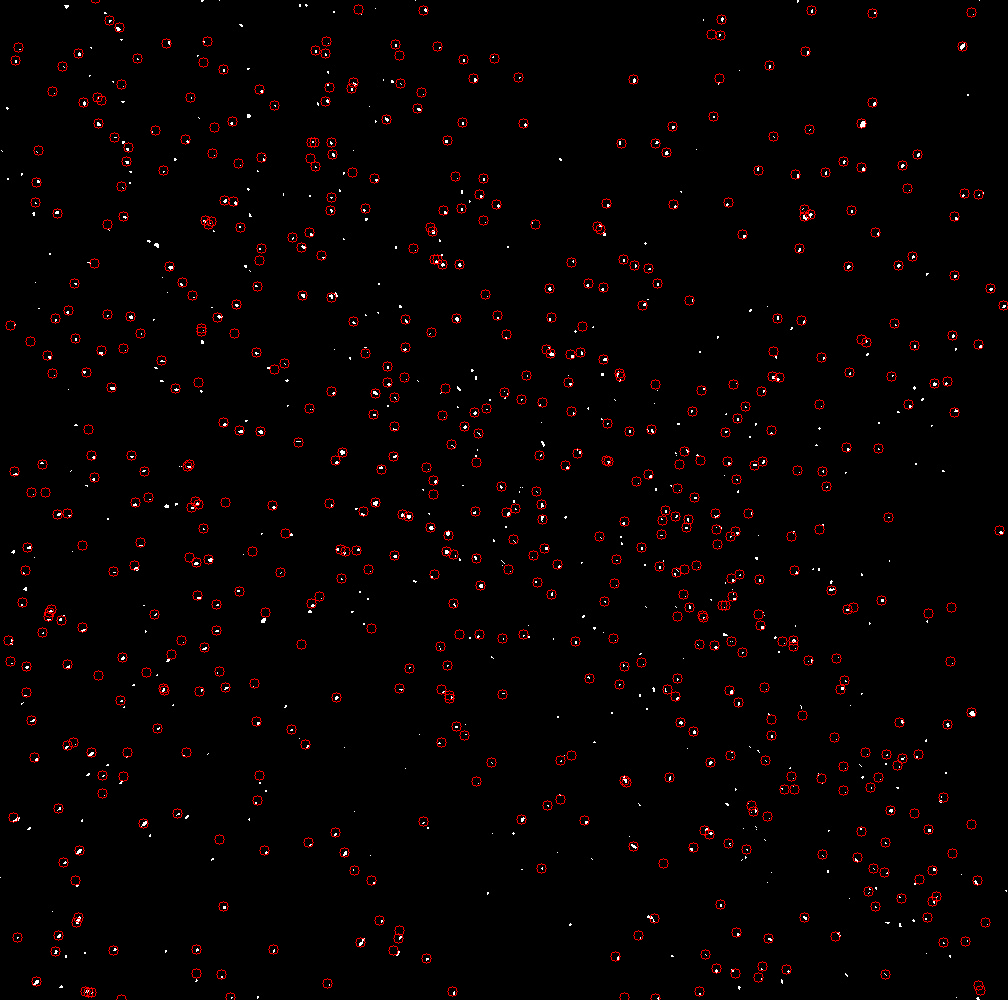
\includegraphics[width=\locateimgsize]{images/locate/iterative-Hough.png}}
	\caption{\centering Iterative concept with Hough backend's result}
	\label{fig:locate:...}
\end{figure}
 \newpage
\subsection{TracTrac}
\label{sec:locate:tractrac}

...

\subsubsection{Algorithm}

...

\subsubsection{Evaluation}

...

% \begin{figure}
% 	\centerline{\includegraphics[width=\locateimgsize]{images/locate/...}}
% 	\caption{\centering ...'s result}
% 	\label{fig:locate:...}
% \end{figure}
 \newpage
\subsection{Hough transform}
\label{sec:locate:hough}

...

\subsubsection{Algorithm}

...

\subsubsection{Evaluation}

...

% \begin{figure}
% 	\centerline{\includegraphics[width=\locateimgsize]{images/locate/...}}
% 	\caption{\centering ...'s result}
% 	\label{fig:locate:...}
% \end{figure}
 \newpage
\subsection{GPU Hough}

The Hough algorithm operates iterating over all pixels of an image.
As such, a new approach was developed, where this loop is replaced by a parallel GPU kernel call.

\subsubsection{Algorithm}

The general algorithm is the same as presented in~\ref{sec:locate:hough}, with all steps executed in GPU.
In particular:
\begin{itemize}
	\itemsep 0em
	\item Step 1 is performed by a kernel, with synchronization after it;
	\item Step 2 is executed by a separate kernel, with synchronization after;
	\item Steps 3 and 4 are run by a unique kernel, that executes non-max suppression on its own pixel, and if it not suppressed, uses atomic methods to add the pixel as coordinate center.
\end{itemize}
On top of the pixels of each frame, also the frames themselves were processed in parallel.

\subsubsection{Evaluation}

The performance of this approach is worse than the CPU Hough transform, both in quality and speed: the algorithm only identifies about 65\% of the bubbles (as visible in figure~\ref{fig:locate:gpu-hough}), running at 17 FPS.

\begin{figure}
	\centerline{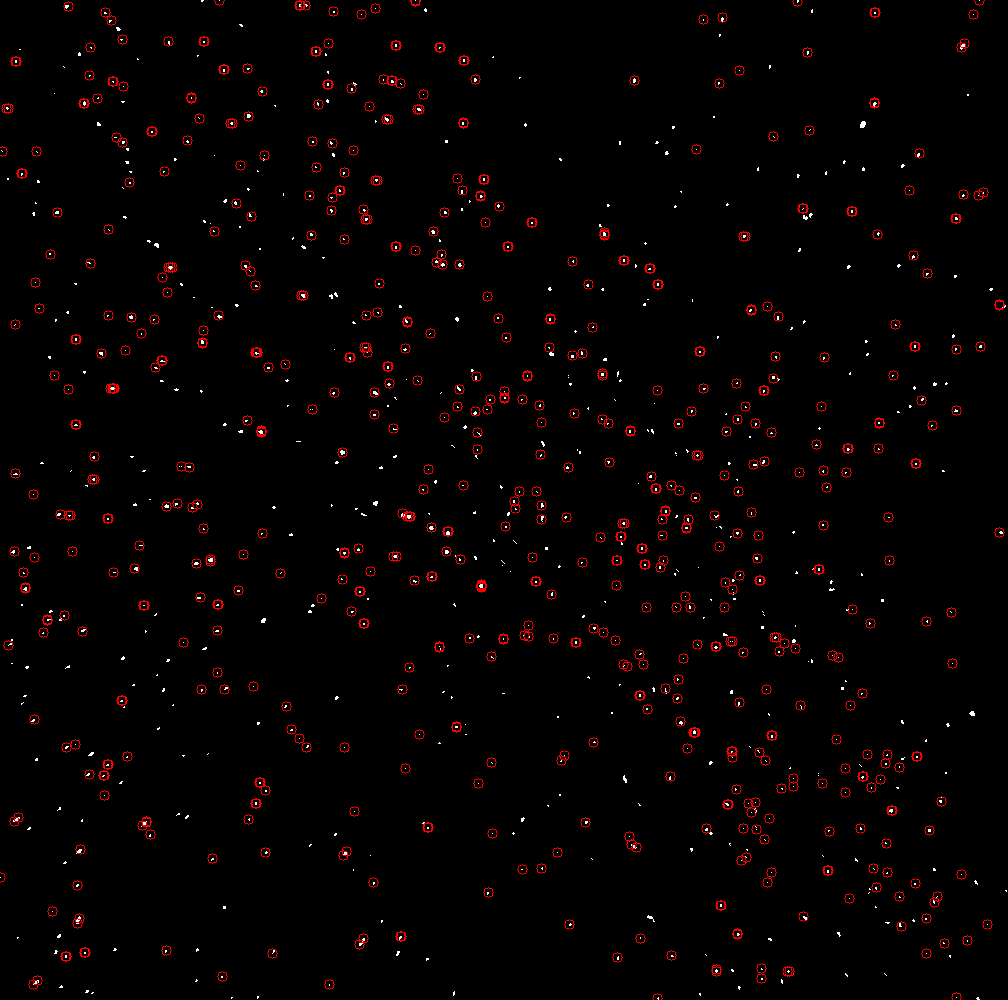
\includegraphics[width=\locateimgsize]{images/locate/my-hough-transform.png}}
	\caption{\centering GPU Hough's result}
	\label{fig:locate:gpu-hough}
\end{figure}
 \newpage
\subsection{4d-ptv}

...

\subsubsection{Algorithm}

...

\subsubsection{Evaluation}

...

% \begin{figure}
% 	\centerline{\includegraphics[width=\locateimgsize]{images/locate/...}}
% 	\caption{\centering ...'s result}
% 	\label{fig:locate:...}
% \end{figure}
 \newpage
\subsection{Image moments}

Thanks the preprocessing done by FPGA, the \locate* task is equivalent to finding homogeneous regions of white pixels on top of a black background.
This task is implemented by the function \texttt{FindContours}~\cite{findcontours} from \texttt{OpenCV}, that finds a rectangular bounding box around pixels with the same intensity.
The precise coordinates of the bubble centroid can be found by computing the centroid (the image moments, see section~\ref{sec:backgr:moments}) of each bounding box.

\subsubsection{Algorithm}

\begin{enumerate}
	\itemsep 0em
	\item Through \texttt{OpenCV}'s \texttt{FindContours}, find all the bubbles for a given frame;
	\item For each region in the output:
	      \begin{enumerate}
		      \item Compute the image moments with \texttt{OpenCV}'s \texttt{moments} function;
		      \item Use the moments of order 0 and 1 to compute the centroids;
		      \item Add the coordinates to the output list.
	      \end{enumerate}
\end{enumerate}

\subsubsection{Evaluation}

As visible in figure~\ref{fig:locate:moments}, the result quality is almost perfect, finding about 99\% of bubbles.
The speed of 67 FPS is extremely good as well, while still being lower than the target.

\begin{figure}
	\centerline{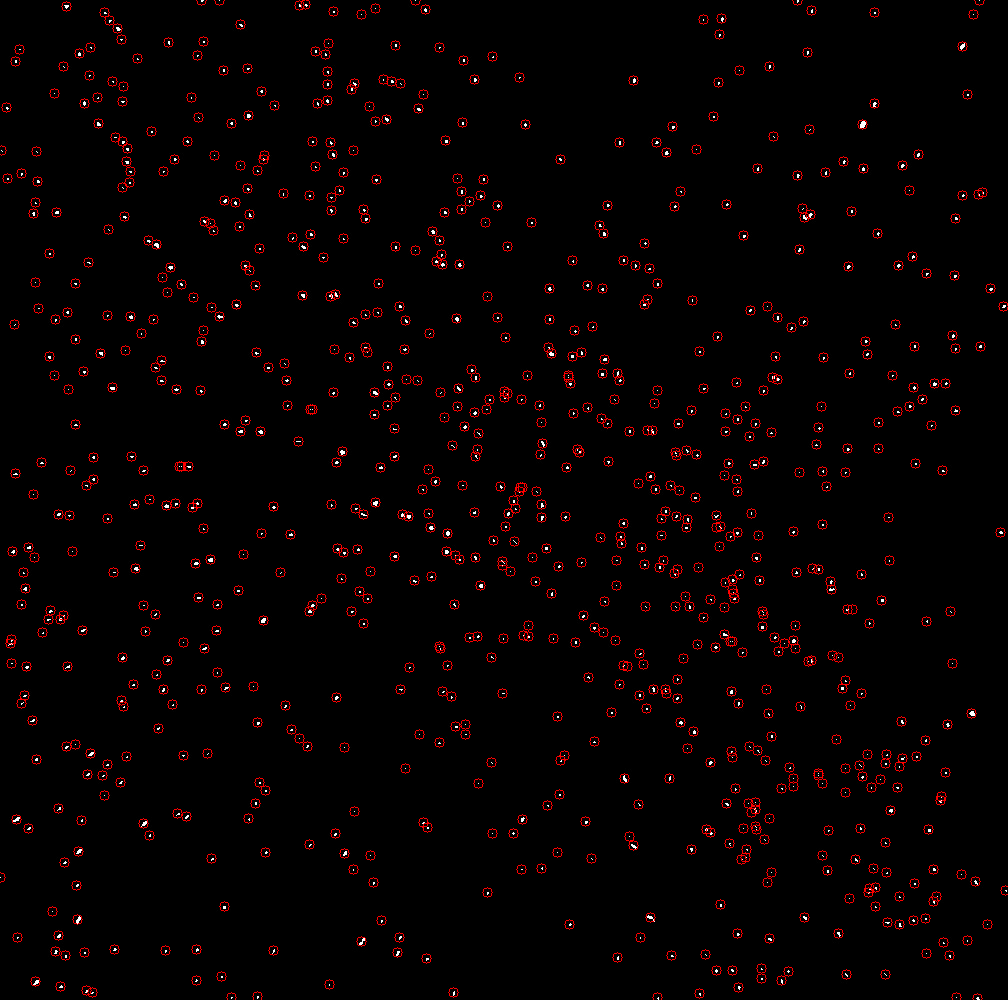
\includegraphics[width=\locateimgsize]{images/locate/opencv moments.png}}
	\caption{\centering Image moments's result}
	\label{fig:locate:moments}
\end{figure}
 \newpage
\subsection{GPU moments}
\label{sec:locate:gpu-moments}

From the previous approach, it was noticed that computing the moments on the different bubbles was a highly parallelizable task.
In fact, the same \texttt{moments} function was called for each bubble found by \texttt{FindContours}.

On top of that, the \texttt{moments} function used to compute moments up to order 3 (for a total of 24 moments), while only moments of order 0 and 1 were used.
As such, a tailored, GPU implementation was created to compute the centroids of the bubbles.
The resulting implementation was also extended to process contours of multiple cameras at the same time,  as well as considering more frames of the same camera in a batch.

\subsubsection{Algorithm}

\begin{enumerate}
	\itemsep 0em
	\item Through \texttt{OpenCV}'s \texttt{FindContours}, find all the bubbles for a given frame;
	\item Find the largest contour among them (this allows all GPU threads to work on the same data size, to avoid diversions);
	\item For each contour found, a GPU thread runs the following kernel:
	      \begin{enumerate}
		      \item Iterate over all pixels, accumulating $M_{00}$, $M_{01}$ and $M_{10}$;
		      \item Use the moments to compute the centroids;
		      \item Add the coordinates to the output list.
	      \end{enumerate}
\end{enumerate}

\subsubsection{Evaluation}

Since the algorithm the exact porting of the corresponding CPU algorithm, the output is the same (figure~\ref{fig:locate:moments}, 99\% of bubbles found).

For the speed evaluation, some tests were conducted to find the best, if any, batch size.
Figure~\ref{fig:locate:moments-cpu-vs-gpu} compares the speed of the CPU algorithm to the speed of the GPU algorithm, with respect to the total number of frames the GPU algorithm processes together.
In particular, this number corresponds to the product between the number of cameras and the batch size per camera.
It is visible that the GPU algorithm is faster, provided that at least 5 frames are processed concurrently, while reaching plateau performance when 10 frames are considered at each iteration.
For the final evaluation, we chose a batch size of 20 per camera, leading to 80 frames processed at the same time by the GPU.

While increasing this batch size adds a delay on the output, this delay only produces a one-time latency, not accumulating over time.
This is acceptable according to the project requirements, which allow for some processing latency, while requiring real-time regime speed.

The maximum speed achieved for this approach was 73 FPS, making this the fastest approach among all, but still not fully reaching the real-time target.

\begin{figure}
	\centerline{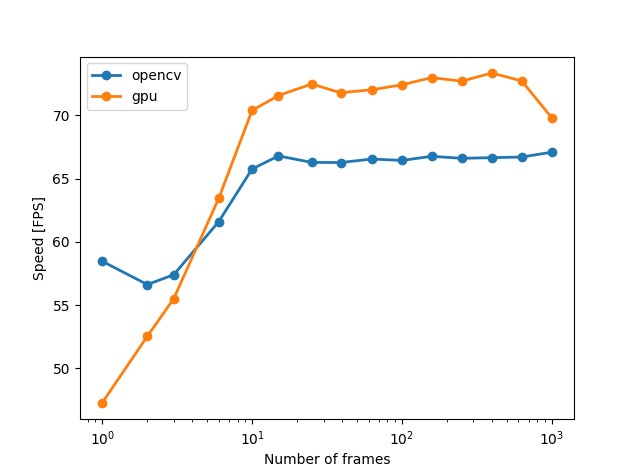
\includegraphics[width=.6\textwidth]{images/moments_opencv_vs_gpu.png}}
	\caption{\centering Comparing speed between CPU and GPU Image Moments algorithms with respect to number of frames processed}
	\label{fig:locate:moments-cpu-vs-gpu}
\end{figure}
 \newpage

\section{Final choice}

All the previously described approaches were compared among each other and with the target speed.
As visible in figure~\ref{fig:locate:speed}, none of the approaches was able to reach the target 90 FPS.
Since no other approach or idea was available, the fastest algorithm (GPU moments, described in section~\ref{sec:locate:gpu-moments}) was chosen.
Incidentally, the selected algorithm was also one of the best in terms of output quality.

\begin{figure}
	\centerline{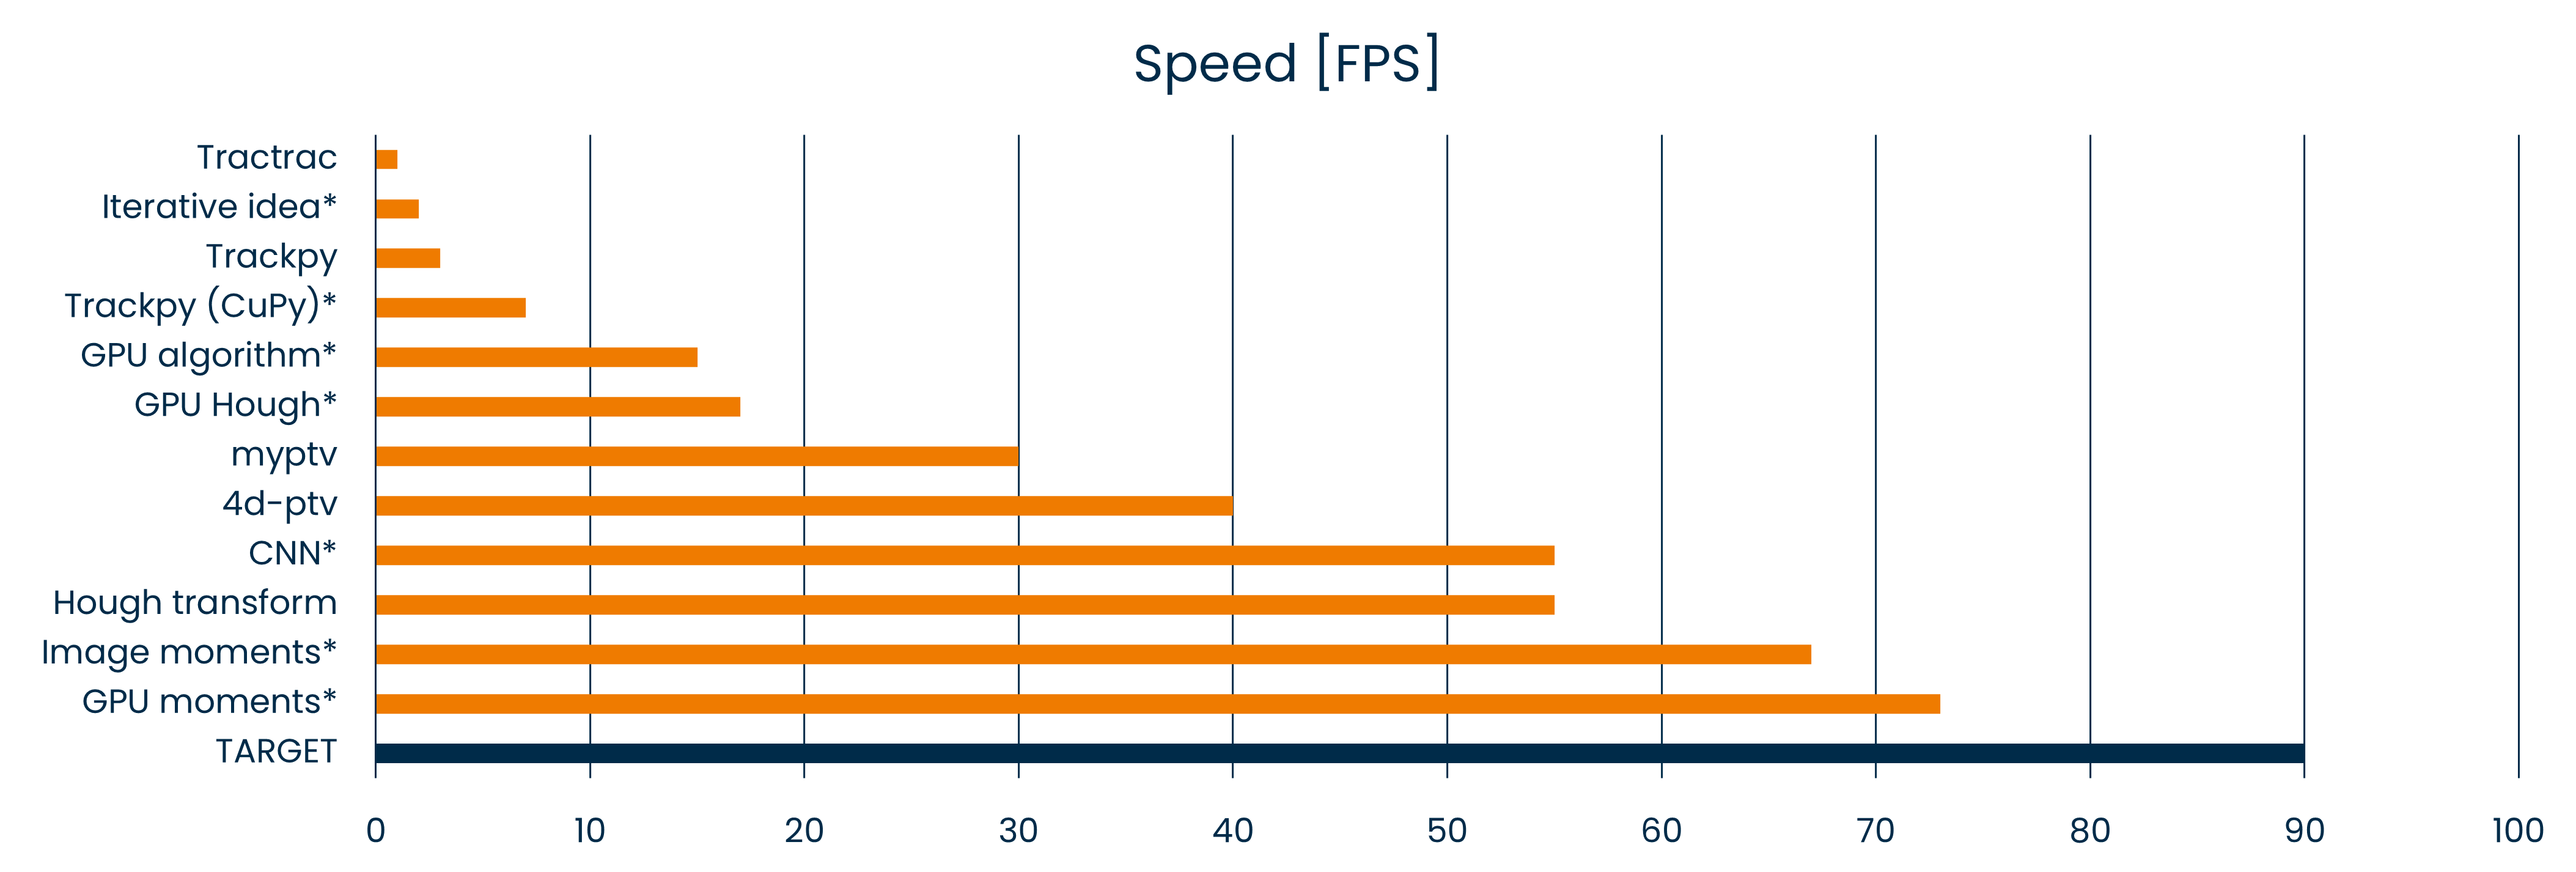
\includegraphics[width=\textwidth]{images/locate-speed-comparison.png}}
	\caption{\centering Performance evaluation of different approaches for the \locate* step}
	\label{fig:locate:speed}
\end{figure}

To compare the different approaches with each other, some modifications were required to ensure consistency, for simpler comparison.
After choosing the final algorithm, it was implemented again from scratch, in order to make it as fast as possible, with no overhead.
This resulted in a decent speedup, which enabled the algorithm to execute at 102 FPS, faster than the target speed, as visible in figure~\ref{fig:locate:speed-cleansheet}.

\begin{figure}
	\centerline{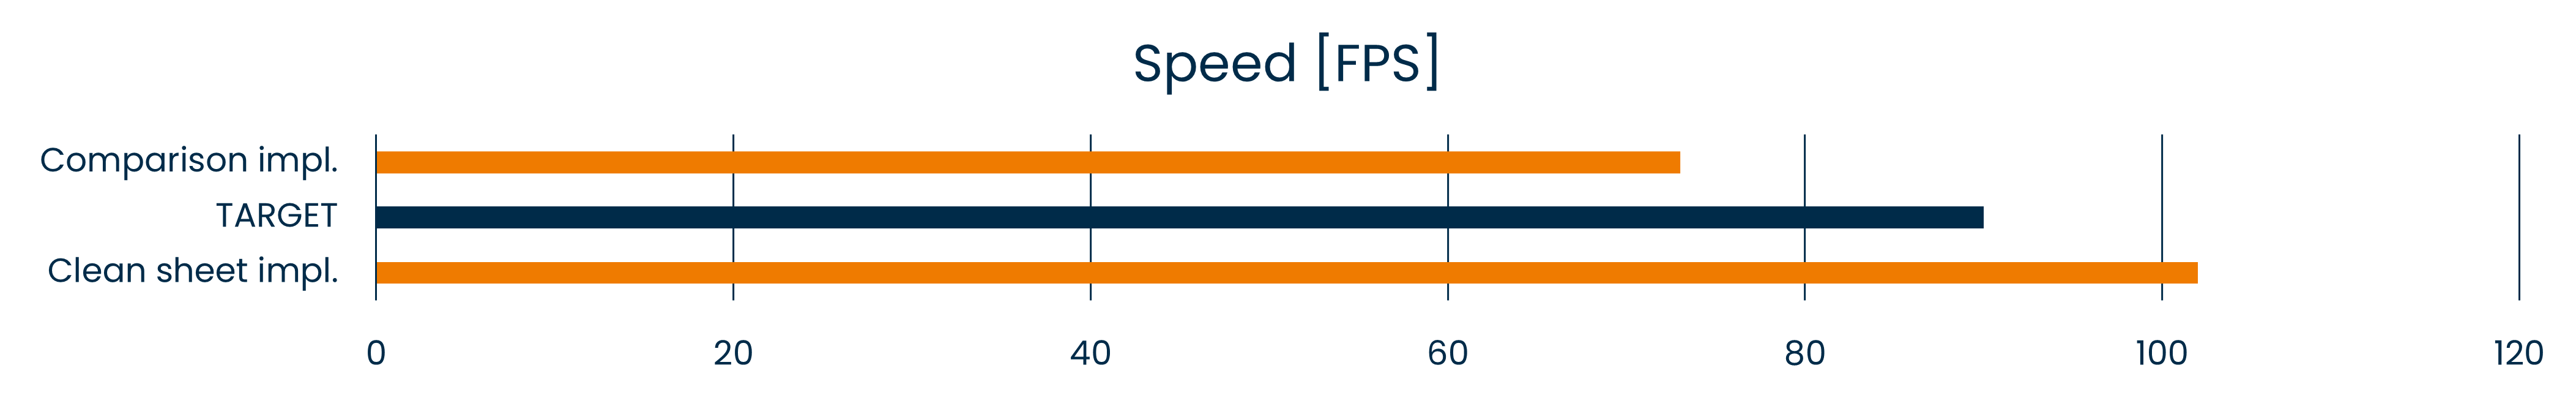
\includegraphics[width=\textwidth]{images/locate-cleansheet-speed.png}}
	\caption{\centering Computation speed of the chosen \locate* algorithm before and after the re-implementation, compared with the target speed}
	\label{fig:locate:speed-cleansheet}
\end{figure}
